\section{2015-08-12 Anchor Interview}

\begin{figure}[h]
\centering
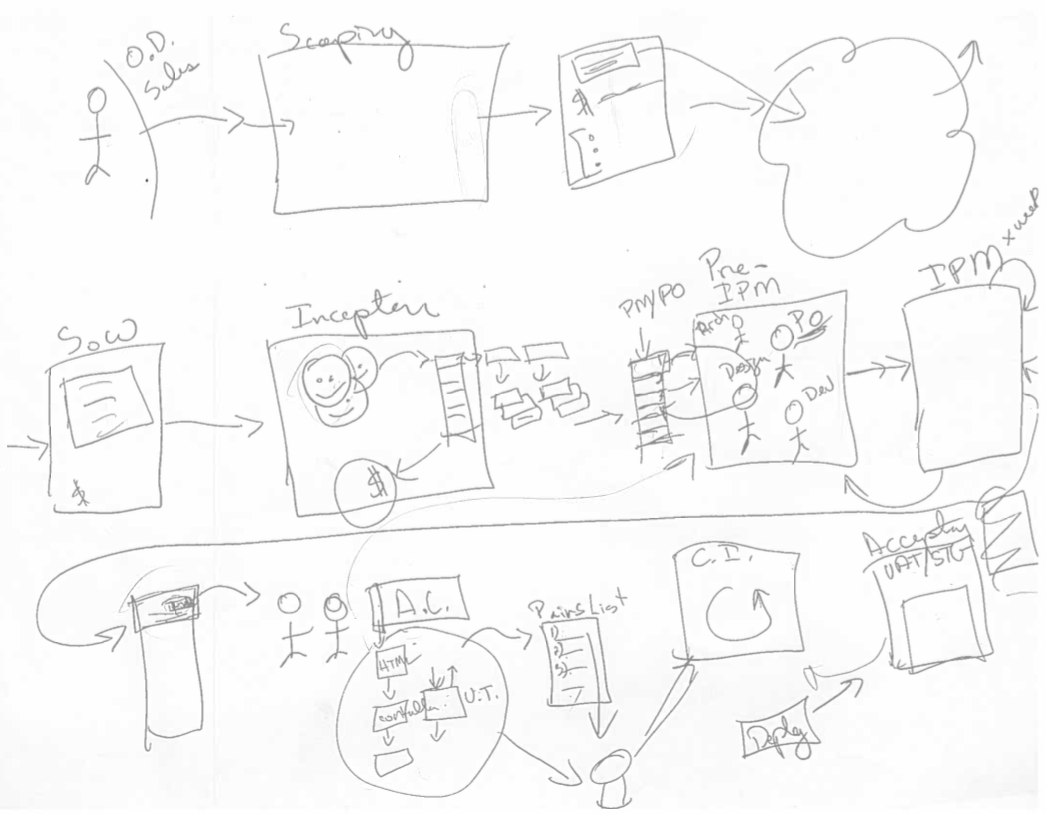
\includegraphics[width=6.5in]{interviews/2015_08_12_anchor.png}
\caption{\quotes{2015-08-12 Anchor's drawing of software development process}}
\label{2015_08_12_anchor}
\end{figure}

\textbf{Todd:} 	So on a sheet of paper, curious could draw your perspective on our process for software development. 0:00:09

\textbf{Interviewee:}  	Our process for software development.  Where do you want to begin?  Or is that like…  0:00:14

\textbf{Todd:}   Really open.  0:00:15

\textbf{Interviewee:}  	So there's a customer, a potential customer.  And they come and there's some kind of vetting to, at least, get them in the door.  We think that they have interesting idea of some kind, and maybe we ask a couple of questions; so this might be the OD or sales.  Just some minimal vetting and then just enough for them to say: \quotes{you know what, I think we could possibly have a conversation about what it is that you want to have built.}  So then we do a scoping with them, and in that scoping, the input is their general idea.  Usually, it's like pretty vague; It could be from very vague to they totally know what they're talking about both on their problem space and with the solution to look like.  So then the output of that is a document that basically tells them this is what it likely is, and this is how much it's gonna cost, roughly speaking, and these are gonna be the roles and responsibilities, this is what you would be buying.  What just really actually, some amount of hours of some amount of people, different skill, that's what we're actually promising and we'll aim for this thing, but we'll always constantly trying to give you the best value thing as we go along.  So that's some kind of proposal, I don't know exactly what we call that, but it is all part of the scoping.  0:02:00

\textbf{Interviewee:}   And then, I'm gonna draw, like, maybe a number of stops here; by the time I see it, somebody signed, like, an SOW or similar that was possibly, like, but influenced by that scoping value but who knows what negotiations or whatever happened after that; and probably informed by that document, like, what we say we're aiming to deliver.  But this is, I think, this is more like a legal document or as the SOW is more like a legal document whereas the thing that came out of scoping is more of like a \quotes{come work with us} and some of the other stuff around that.  So then, we go into an all of these assumes it's ok.  I'm talking happy path.  Cool?  0:02:59

\textbf{Todd:}  	Yeah, I'm good.  0:03:00

\textbf{Interviewee:}  	So then we do an inception, and this is where, regardless of what we said over here, we get them to get really clear about who is the person that they're targeting; like, ok so it's about a product market fit, who's the market, what's the product gonna be.  So here's this person or persons or personas, and then for each of one those, like, what are the kinds of things that they need to get done, right?  So they've got things that need to happen, that ultimately will result in to some kind of outcomes, and it almost always like it's gonna convert to dollars in some way, shape, or form.  Sometimes it's a non-profit thing and that's slightly different, there's mixed motivation.  So then what we do is we say, \quotes{ok, in order to meet those tasks, what we need is features from the product} and so we're calling out, like, epics, if you will, feature sets, whatever, and then when we start breaking those down into individual stories and these are just sketches at this point.  We're not gonna get all into acceptance criteria right away, it's just like trying to enumerate coz really the outcome of the inception is a backlog. 0:04:43

\textbf{Interviewee:} So you've got some product owner, who culls the outcome of that into a prioritized list of stories, each one of those describes at tiny interaction between this person and the software that we're building.  Ideally, there's variations on that but then, so that's what an individual user story is.  0:04:58

\textbf{Interviewee:}   And then we go to kick off.  So then, we have our first iteration planning meeting where we take as input the prioritized backlog and for each story we go through them.  And by then, the product owner has got them into a point where I call it readied, they've met the definition of ready, which is they have clear acceptance criteria.  There might even be, a pre-IPM where that work is done, as well as, so this is the input is the backlog and the output is the backlog in the pre-IPM.  There are two things that happen, one is that we get clarity early on what the requirement is, and the other is that we get technical input to help with that prioritization and viability, like, ‘ok this may seem simple, like on the face of it', but actually, there's a whole of things that has to happen to make that work, etc. So we surface some of that, the pre-IPM includes somebody from the product side of the house and someone from development, so product owner, development.  Sometimes depending on those, the story can get more complicated, the more requirements, with the greater the variety or the more exotic the product is.  So you might even need someone in from design who is kind of help guiding how this should unfold and the interactions between things because there's all kinds of decisions from that end.  I Imagine, although, we haven't done this yet, in an enterprise client that you might even have somebody from like architecture there, business architecture.  The point of this conversation is to get all of the perspectives that need to be folded into the prioritization and the validation of, that the stories are legit.  0:07:11

\textbf{Todd:}  	Yes.  0:07:12

\textbf{Interviewee:}  	So then that goes into IPM, and this is a straight-forward roll through - the from top to bottom - the backlog, and we go over each story.  We read out title, we read through the acceptance criteria and then the team points each of the stories, the purpose of that is to surface complexity and to get a general, like, understanding, like, common understanding of what this thing actually is, what it is, what's gonna be involved to building it.  0:07:52

\textbf{Todd:}  	Yes.  0:07:53

\textbf{Interviewee:}   	We don't give in to like, we try not to give in to implementation details.  Sometimes, we have to dip down for a second to like verify that we're all speaking the same language, that we're all really envisioning the same kind of thing.  But that usually is surfaced by like, \quotes{I pointed at one and you pointed at five,} and then I would like \quotes{what?}  So then that hopefully prompts a conversation.  If we all said three, it's good enough for now we move on, if we all think it's about the same thing and the product owner doesn't lose their mind hearing that number, then we're all kind of okay.  Then the output of the IPM is individual points on the stories, and we typically go for some amount of horizon so the minimum that I feel comfortable walking out with is at least for the week, so we don't have to, like, break the flow of getting work done before the next IPM because we're gonna do this once a week, these IPMs we're gonna do this once every week. But ideally, a little bit more runway so that we mitigate against that the team haven't jumped out of the flow and also to, like, help the product owner have some room to sort of steer.  If they only have so many points in the stories, then they have to kind of pay the price of reprioritizing. So that's IPM.  Haven't have written a line of code yet.   So then, after IPM, we get working. So out of the backlog, a pair picks up a story and so then that pair looks at the story...  How deep do you want me to go, because I can go all the way down to like testing and stuff.  0:09:48

\textbf{Todd:}  	Sure.  0:09:49

\textbf{Interviewee:}	Ok.  0:09:50

\textbf{Todd:}	This is your diagram.  There's no wrong answer.  0:09:54

\textbf{Interviewee:}  	Alright. Ok.  So, the pair looks at the acceptance criteria and they say, \quotes{hmmm.... what test do I need to write that will help?  Or a set of test that will help if those tests ran green?  I feel really confident that we've met the spirit of that story.}  So they start there.  Usually at pivotal will do typically outside in so that means if we write something that looks like an acceptance test, something that describes very closely what this person with the persona experiences both in what they do, and what they see back from the software.  So we write the starts, we start with a very low fidelity version of that. It's not gonna describe the whole interaction, it might describe the smallest piece of we could possibly articulate; so we start there.  And then we run that test and it fails.  Then we say, \quotes{hmmm, ok, so we're in this architecture, what's the next part that we need to build in order to begin to meet those needs?}  And we work our way down the architecture.  In a typical web app, there's something that's displaying, an HTML page, and then there's something that is probably orchestrating the generation of that HTML, like a controller and usually we try and separate our concerns. We think about these things as we work our way down driven by trying to meet just this one acceptance test.  0:11:26

\textbf{Interviewee:} So along the way what we do is we write individual unit test for the components that have interesting behavior.  The controller does have interesting behavior.  It takes in some input and it makes some decision about what should be the output, what should be the resulting HTML.  And that controller also interacts with other collaborators.  So we have tests that say, are you properly handing off these parameters?  So these really fine-grain unit tests. But the key is that these things are, each time we write these tests, we're setting an expectation on that little tiny piece of the system, in the same way that our acceptance criteria are setting an expectation on the software, and our user stories are setting expectations on the feature .  So forth, all the way back up. We're trying to be needs-based  all the way down as we do this; that's probably good enough.  The details of how that happens varies wildly and even like within this, there are different schools of thought about how that happens.  There's people who believe in writing units for every little thing and people who say \quotes{no, you can set certain bullwarks} and write tests around the bullwarks.  Let everything sort of float in between.  0:12:43

\textbf{Todd:}  	It's a whole like, Chicago versus London.  Like, on how much mocking and doubles do we have?  0:12:49

\textbf{Interviewee:}  	That's right.  0:12:50

\textbf{Todd:}  	How much more integration of the unit test level do we have.  Are we really testing real things or not.  0:12:55

\textbf{Interviewee:}  	Yes, exactly.  0:12:56

\textbf{Todd:}  	Yeah.  0:12:57

\textbf{Interviewee:}  	Exactly.  So and the other part, too, is I think a factor in there in the choices that I make about these things, have to do with who the team is.  On like what their level of experience with test driven development is, and if it's really, really low, then I'll tend to want to have them write many more unit tests.  And I know that that is more fine grain tests, I know that that's harder at first but then they more quickly ramp up because they have more guard rails around them to guide them along their way, as they're learning the knack, the feel, the tacit experience of being test-driven.  Then as they start to become more comfortable, we can back off a little bit on some of these unit tests; especially if they're not catching anything, so test have a shelf life and if they haven't caught a defect, then there's a question of whether or not it's actually carrying its way.  So that can be a way of starting to prune part our of test system.  0:14:10

\textbf{Todd:}  	There's a bunch of people who are concerned about declarative tests or tests that test declarative code.  0:14:16

\textbf{Interviewee:}  	Ooh. Yeah. 0:14:17

\textbf{Todd:}  	Do you worry about that when you're thinking about this?  Difference is Rails has a lot of configuration and it's like why test the configuration when we already know that Rails works.  0:14:26

\textbf{Interviewee:}  	Right.  0:14:27

\textbf{Todd:}  	And that's through another framework to like... 0:14:30

\textbf{Interviewee:}  	Yeah.   0:14:31

\textbf{Todd:}  	Or does that not really end, you just like, \quotes{hey, let's just test everything?}  0:14:34

\textbf{Interviewee:}	 No, it does matter.  And I don't know that I have like a pat answer.  I think I'll probably flip flop depending on my mood and who knows what else.  I think if it's something where it is like a one-time configuration, so some of the factors are “how often are we gonna touch this;”  “how bad is it if we get wrong?” If it's like important plumbing that could get broken later on or something like that.  Coz you can do bindings, right.  Like bindings are kind of declarative piece so you tests those.  So I'd start off probably testing that kind of stuff.  But I'm not gonna test to see that configuration params are correct.  0:15:36

\textbf{Todd:}  	Because presumably it won't start up if they are wrong.   0:15:40

\textbf{Interviewee:}  	Exactly.  0:15:41

\textbf{Todd:}  	I interrupted you.  Did you finish with your diagram to the very end of the story?  0:15:45

\textbf{Interviewee:}  	So we get through the story, and then there is more to this process here.  As we go along through this development, some things feel easy and flow well and some things don't; and the things that don't, they go off on, what I call a pain's list, and I learned this from George Dean.  The idea is that let's enumerate things, let's just quickly note things that are challenging.  We may even have to work around them, like, \quotes{ah I want to take this certain tack but I can't,} so we note it.  And then, what I'd like to be able to do is get to the point where I can click finish on my story in Tracker.  But before I do that, when I feel like I've met all my acceptance criteria.  All my acceptance tests have met the acceptance criteria, then we'll stop as a pair, we'll quickly triage this list, some of the items just suck and we're not gonna do anything about it right now.  It's probably just, it's something that, it's not worth calling out as a chore yet. Or maybe it's too big, too; or maybe now after having gotten through the story, maybe we've changed our mind, maybe we have different perspectives, something like this.  We'll do one of three things with it, one we'll either address it right now, like \quotes{you know what, this is a two-point story and my god we flew through this, it took us an hour or two. Let's say we've been tracking a little bit longer for those kinds of stories.}  I feel like I have a little bit of buffer in terms of raising the quality dial a little bit so we'll address a pain.  What we're trying to do is hit the thing that's gonna be the least of effort for the most bang. We're looking at things, there often things like, it's all about maintainability, making the software more of an asset than an expense.  So readability, where there's something that's different for no good reason, bringing that back in line, all those kinds of things, so we'll address it - that's one option.  Two, we say, we're not gonna address it now but it's pretty important; it's one of those things where this is really gonna bite us if we don't do something about this or it's gonna create a ton of back flow where we will be blocked a whole bunch of stories if we don't address this soon.  So we'll mark it as a chore.  Or three we say, \quotes{yuck, don't like this.  It isn't necessarily gonna bite us right now, and if it really is painful, we're gonna discover it again}, so we delete it.  We try to empty our pains list and that's the last step and then we go and we click finish.   0:18:49

\textbf{Interviewee:}   As a part of clicking finish, either, and I've seen this in many different ways, either it's automatically hooked up from our version control system in our CI, we have a CI box, some CI setup that's listening to the same repository that our code is going into and it kicks off a build and when we commit with a certain message, it will mark it as, it will click the finish button for us effectively, finishes and then the tracker story number.  0:19:33

\textbf{Interviewee:}   Meanwhile, and this next step might have happen as a part of this whole development process. As long as everything is running green, I could actually commit and I'm not delivering a feature that couldn't be deployed, so maybe partial but if it's not seen, then it is ok.  So anyway, my point being that, we have a continuous integration server that acts like the nth + 1 developer on the team.  So it goes and it fetches the code just like the developer would.  Actually, the initial version of this was called integration station, where it was literally a box at the end of, like an end cap on a team's desk, and you'd get done, and you'd walk over, you‘d manually do this process.  And now it's automated.  The point being that we're demonstrating that the code can be built from scratch reliably from master.  Which means it's included in everybody's work up to that point and then all test runs. 0:20:39

\textbf{Todd:}  	Nice.  0:20:40

\textbf{Interviewee:}  	Ok so when we click finish, we see the CI build go green, then this varies also wildly.  We wanna deploy to some kind of acceptance area; so maybe it's called UAT somewhere, sometimes it's called staging, whatever it is.  So it's a non-production environment that now, the product owner can go and vet that feature against the story, thinking about this person and getting their job done.  So that can either be accepted or rejected; if it's rejected, then it goes back into the backlog.  And then, I didn't really make enough room for this.  0:21:34

\textbf{Todd:}  	If you need to use a second sheet, you can.  0:21:36

\textbf{Interviewee:}  	Ok, Cool.  So let's go like this.  So that's where the acceptance happens.  And then time passes, so we go about for a week and then we get together as a team and we dead reckon, at the end of the IPM, it's almost sort of like we all sort of have an idea about where we're going and what we think we're gonna accomplish.  0:22:02

\textbf{Todd:}  	Yes.  0:22:03

\textbf{Interviewee:}  	And then wind and weather, like, affect our actual location where we end up, so we need to, as a group, see where we're at, both in terms of progress we've made in development of the product and what we've learned along the way in terms of working with each other, and the technology that we're using, and what we've learned about the product and all these stuff.  It's navigating in all these dimensions so that's what the retrospective is about.  And so there, we step out of getting things done mode and trying to into a mode of dis-identifying that and reflecting on the process.  And we have kind of a pat way that we sort of do it at pivotal, there's a lot of different ways to retrospect.  But we focus typically on emotion-based sense-making.  So we say, what makes you happy, what leaves you sort of neutral, what might make you angry or frustrated or whatever.  That's a terrific way of getting an idea about, like our emotions are a really good way of developing situation awareness so we're gonna have one way of doing it, it's probably the best way that I would know of.  So we just throw up a happy face, a middle face and a frowning face up the board. We have people register anything. You could just be having a catharsis in front of the group, that's fine.  The point is to try and make some sense of what just happened just this last week.  And ideally, we come up with action items; and these could be in the form of what actual people do, so \quotes{oh, so and so needs to add a chore,} or we need to change this like about how we, the time that we do our stand-up or something like that, or they could be team agreements, so we clarify what the definition of done is.  Don't click finish until you see it, you smoke it yourself in the staging area before you hand it off.  Or please include instructions in the user story about how the product owner should accept this.  Some sample data or whatever it is.  We come to try, we looking to continuously try to improve as a team.  And that's the moment where that happens.  And then ideally, you kick the whole process off by jumping back into an IPM away we go again. Ideally, along the way, in parallel, this collective, this little mini team here is keeping the backlog groomed, looking ahead trying to think about, again, dependencies to both end.  What's important, what needs to get done in order to make a story successful and then rinse, repeat.  0:25:00

\textbf{Todd:}  	I think I got it.  Anything more that we need to add to this?  0:25:04

\textbf{Interviewee:}  	Let's see if there is any major pieces missing.  Now, I said happy path.  0:25:16

\textbf{Todd:}  	Yes.  0:25:17

\textbf{Interviewee:} 	So there is one fork off that can happen, way up in the front, you know what I was saying, the OD or sales or someone could be vetting the customer, now could very well be that they just have no idea, they're totally barking up the wrong tree, or they're asking us to do stuff that are just so out of what we do, that we direct them to somebody else or we try to give them some feedback, that like, you're not ready for this.  Or it's not a good fit.  Another possibility is they're actually kinda close, and if they can get a little bit of help of defining what it is that they want, then we can maybe get them there, that maybe we can get them in a room and actually do a valuable scoping.   And so what we do is offer them a Design and Framing.  And this is where we take them through a workshop where we help them unearth what they do know about their market and their product and start to explore their business model a little bit, and try and talk about, get them to think out loud about what they do and don't know about that. There's a sort of like exploration phase of it.  Ideally, what we're doing is getting all this complexity out of their heads on to the table and we then try and help them converge on, prioritize and focus, force them through various types of focusing exercises to really get down to like, what is the most important part of their business right now.  0:27:02

\textbf{Todd:}   Yes.  0:27:03

\textbf{Interviewee:}  	Get clear on what you know and what you're speculating on and what you need to know.  Like get into like, what do you need to learn kind of thing as supposed to how much money you need to make kind of focus.  0:27:16

\textbf{Todd:}  	So if I understood you right, it sounds like the DNF was mostly for the unhappy path.   0:27:22

\textbf{Interviewee:}  	It is \ldots  0:27:23

\textbf{Todd:}  	Could you see people in the happy path needing that?  Maybe I misheard you.  0:27:28

\textbf{Interviewee:}  	Yeah, yes.  0:27:33

\textbf{Todd:} 	Maybe think about your own projects.  How many of them do you think should have a DNF at the beginning of them?  0:27:40

\textbf{Interviewee:} 	So let me see.  So we did one for Sundance, it was one of the first.  Yeah, so and as an anchor, I haven't been involved in actually any of them that's been on the project.  So that's one big gap, like, in the same way that we should have a balanced team sitting in the pre-IPM, early up in this phase, it's I feel like we could do better in terms of getting all the voices in the room.  Or at least having some continuity of context.  0:28:25

\textbf{Todd:}	  Having engineering involved in the DNF sounds beneficial.  0:28:30

\textbf{Interviewee:}  	Yeah, yeah. And it's not just that they're participating, there's context that happens.  In the same way that part of the value of pairing is not just what design decisions were made, but those that were discarded and the reason why they were discarded, like why we didn't go down this path.  There's lots of context to be gained, understanding a more refined meta model by participating, being directly involved and hearing exactly how people are expressing themselves and seeing the connections between the people and things in that level of discussion in that business model discussion.  0:29:10

\textbf{Todd:}  	Ok.  0:29:11

\textbf{Interviewee:}  	So, it's not just that there is somebody there with that expertise I think it's also that as we move into the execution, the more that the people who are doing the work can understand that, then they can make better choices in the trenches.  0:29:27

\textbf{Todd:}	I think for me I thought of the design and framing is, if you have a client that doesn't have a clear understanding of what they wanna build, they may think they do.  Or it's too big to do one engagement and it seems to me like a good pre-filter to the engineering cycle before you have expensive engineers on this thing writing code.  Just really make sure and validate that we're building the right thing.  And we actually understand the user that we're building it for.  0:29:51

\textbf{Interviewee:}	Right, yup.  0:29:53

\textbf{Todd:}  	So I'm really intrigued by the idea, is this a normal sequence or is this when we have, like, a client that's not a good fit and we're trying... you know what I mean?  0:30:00

\textbf{Interviewee:} 	The way that we've talked, the way that I've heard it framed, it's when the client is, like, one step away from being ready.  0:30:11

\textbf{Todd:}  	Interesting.  0:30:12

\textbf{Interviewee:} 	And what we're trying to do is help them get that additional level of clarity so that they can get into the room and scope so they can actually articulate software features so the rest of this process can run.  0:30:24

\textbf{Todd:} 	Now, just to clarify. For me when I think it ready, I think maybe when they have their own usability team, design team, they might have done all the things we would do, then they're for the ready. But listening to you, maybe ready means something different.  0:30:38

\textbf{Interviewee:}	So, at a bare minimum,  it's that they can articulate what features they want in their software and that they have some kind of plausible story for how investing in that is gonna help them yield their goal.  0:30:58

\textbf{Todd:}	If they have that they're ready?  0:31:02

\textbf{Interviewee:}	Yeah, I think that's the criteria we've been using to get there.  0:31:09

\textbf{Todd:} 	<interrupt> Okay, this is helpful for us.  0:31:10

\textbf{Interviewee:} 	We've been using to get there.  0:31:12

\textbf{Todd:}	Nice.  0:31:14

\textbf{Interviewee:}	Yeah, that's my understanding.  0:31:15

\textbf{Todd:}	Ok.  0:31:16

\textbf{Interviewee:}	Whether or not, that's actually, coz I'm not the OD, I'm not in sales, I'm not purview to those vetting decisions but I hear about them.  0:31:30

\textbf{Todd:}	So we're talking about exception paths. Are there other negative flows?  0:31:36

\textbf{Interviewee:}  	Let's see.  Well there's sort of some obvious stuff like contract negotiation, someone gets kicked out because, \quotes{oh my god, you're that expensive?}  Didn't you read the price sheet? Let's see there's that... Things can happen like where we inadvertently discover later on the process, so like \quotes{oh wow! We are so not ready.}  That can happen.  I can't give you a specific example where we went into an inception and had to abort; but I've been in a couple of scopings personally where we kinda thought things are sort of new and then we got into it and as I started talking about it in more depth, it was like, \quotes{oooh yeah.}  For one reason or another, they didn't appreciate yeah, so there's that.  0:32:49

\textbf{Interviewee:} 	All kinds of things can happen in a pre-IPM, you could like clear the decks, like \quotes{oh my god, we're working on the wrong thing when you should totally work on this thing.}  That can happen.  It doesn't necessarily go linearly, well IPMs can go off the rails when we haven't done a good job in clarifying and, like, getting the stories to meet the definition of ready.  There's all kinds of back flows that can really kind of like this is a crucial piece like in terms of, like, actual production itself.  You can get back flows anytime, there is an invalid assumption or worse, un-surfaced assumption. And those can be off effectively kick backed into a pre-IPM state, if you will, mark the stories as blocked and move on.  In the software development experience itself, like you're wrong 99% of the time, and then until you're right for the 1% and then you run into the next wall.  There's constant back flows. 0:33:54

\textbf{Todd:}  	Right.  0:33:55

\textbf{Interviewee:} 	See our builds will fail every so often even if you're super diligent, that just happens; and there's to the extent that configuration is not automated and some things like migration or change in dependencies or things like that.  Things can fail in acceptance as well and those are backflows; but they're not horrible exception cases.  0:34:32

\textbf{Todd:}	Fantastic.   0:34:35

\textbf{Interviewee:}	Yeah.  0:34:36

\textbf{Todd:}	This is very similar to the way I think of the way we develop software.  It's nice to see you draw it out this way, so thank you.  I have so many questions I wanna ask.  I can't contain myself.  I'll resist all my questions, and I think this is a good one for us right now.  When you think of the current project you are on, what are some of the challenges that you're facing?  Either as an anchor or as a software developer or as a pivot for the project?  What makes this project special or unique?  What's the pain points that you're feeling?  0:35:15

\textbf{Interviewee:}  	Ok, right now, our biggest pain point is that we're in a halfway state type engagement with my current project.  What started out as a unified team, had to split into 2 teams because someone with a lot of influence came in to lead, lead part of the team.  He does not, at all, see the value of an iterative incremental approach to software and just kind of like down the list.  Everything we do, like, it just doesn't compute for him.  And he's been very successful from his perspective at doing it the way he does it.  And so we had to split off a separate team that is working in an XP way and so we're doing development separately from this other team.  So the biggest pain point around this is the clarity about how much are we… coz we're consulting, we don't just develop software, the whole point of why people come to us is to enable them to do it themselves.  0:36:42

\textbf{Todd:}  	But he doesn't want to do it the way we're doing it.  0:36:44

\textbf{Interviewee:}	Oh, no. and everyone else on the team could totally go with it.  0:36:49

\textbf{Todd:}  	Go with his way?  0:36:50

\textbf{Interviewee:}  	No, go with our way.  0:36:51

\textbf{Todd:}  	Oh, ok.  0:36:52

\textbf{Interviewee:}  	But he is so influential, politically, like organizationally, he gets to come in and totally dictate like, this is how it's going to be done.  So there are moments where, even the product owner, like, wants to...  He has seen, the product owner has been, lived through, been a product owner on a pivotal project – multiple.  And he says, "I know what it looks like, I know what that flow is, it's amazing, I want that.  But I can't do it because of this guy."  He is acting like the technical lead, he's a business architect.  At least he's coding, but it's this chief surgeon style, so  everybody has to surround him and he holds the whole architecture in his head and the rest are billings (?) and scribblings and he doles them out in terms of tasks.  So it's very much like centralized approach there. And so there's even this desire to like, \quotes{hey can you help us be more test-driven even if it's hard to do that in this platform.}  This guy says we have to do it in.  Where the team is programming in XSLTs and a little bit of Java modules around it, and he built up this huge universal business widget adapter that takes any possible XML message and can apply any number of XML transforms and can then output to interact with any kind of end point.  It has this event model engine.  The whole thing is just like a Rube Goldberg type, it's amazing.  They're getting it going and the thing is... I'm getting off track...   0:38:43

\textbf{Interviewee:}   The pain point is that there are these interactions along the way, that's in a retrospective or even moments like we had an IPM where they...  Somehow the product owner was able to convince this guy to at least stop using a spreadsheet to track tasks and make them chores in tracker. So at least there is some hope of having something that you can prioritize and move around, that there's some visibility outside of this spreadsheet that's updated regularly etc.  So we just naturally me and the guy I'm working with, kind of co-anchoring, we just naturally said, we took the first story and said ‘how do we know this is gonna be done?', because it was just a task.  So through, we rotated these things 90 degrees so that they have acceptance criteria, that they have outcome language around them, instead of output language.  That was like all these consulting that we would normally do; if you see a backlog gone sideways, like, that's what you do. But it's unclear whether or not that was actually part of our engagement, because, they're like a separate team.  The pivotal product manager was out for the week and so as co-anchors, we filled in for him.  0:40:04

\textbf{Todd:}  	Was that appreciated?  0:40:07

\textbf{Interviewee:}  	The product owner was, like, delighted.  And I think that we... 0:40:12

\textbf{Todd:}  	Feel free to open that thing (Kambucha bottle).  0:40:14

\textbf{Interviewee:}  	I'm just trying not to not make a mess.  I think I'm just gonna commit.  0:40:19

\textbf{Todd:}  	Yes, you did it.  0:40:20

\textbf{Interviewee:}  So he was delighted and there's actually a program manager that is overseeing all of the development here for Corelogic.  0:40:37

\textbf{Todd:}  	No, oh no. I'm putting 2 and 2 together. (This company is trying to adopt the entire pivotal way of working for their entire company, but there are clearly people there who do not embrace this approach to software development.)  0:40:50

\textbf{Interviewee:}  	Ok.   0:40:51

\textbf{Todd:}  I think this architect might feel threatened by the way we work.  It's just the sense of value, he would feel very...  0:41:09

\textbf{Interviewee:}  	Who knows what's going on in a person's head?  0:41:12

\textbf{Todd:}  	Then we have whole team and code ownership and all these things and if all of your value comes from being the chief surgeon then another way of working might be scary.  0:41:24

\textbf{Interviewee:}  	And yeah, it's, hard to know. I mean, how, exactly, is he responding to it?  It might have flipped  the bozo bit, you know, for him for all. He may have decided early on, well, this is all well and good for start-ups but I'm doing enterprise software here and you don't increment your way to high volume message processing.   This is industrial software, you architect this thing.  It may not be that he feels threatened, it may that be he firmly believes the way that he's approaching is the appropriate way to approach it and that because he hasn't had that experience of what it's like to navigate his way through a project, that he doesn't have faith that it can be done.  0:42:21

\textbf{Todd:}  	So how do you find yourself tailorizing this process?  If at all, to handle the situation? 0:42:30

\textbf{Interviewee:}  	First of all, hats off to Mr. Gerhard and Bearnek because they… so Mike Gerhard was the anchor before myself and Mike Bearnek came in to help out.  What they did was they helped define: this is your dance space, this is our dance space, this is what we are on the hook for, this is the process by which we're going to take your hundred page architecture document and find ways of getting in to a scoping so we can to the pivotal process.  So they helped create lots of clarity in terms of that. We will be in a world of hurt if it weren't for them.  And so we have this piece that we're developing, that's the web front end to this message processor thing, so the pieces that we have those interactions like what I was talking about was mostly like our PM is having to figure out how much of his time is he gonna spend as a glorified secretary  versus actually showing process. And it's every so often there's, so let's see, from my experience is... how are we doing on time?  0:43:46

\textbf{Todd:}  	Doing good.  0:43:48

\textbf{Interviewee:}  	So my experience around all this is there are a few people that are on that other team that periodically have an opportunity to cross over and they get to pair with us. And we just like put out the red welcome carpet, any moment you want, we can split our pair, like we're ready to go and every time they've come over, we've just accommodated them.   And we had a couple of really good pairing sessions.  But these are also like key technical folks on the implementation of that processor piece as well.  It's far and few between and they're just getting crumbs it terms of experiencing the whole flow.  0:44:33

\textbf{Todd:}  	Coz the whole company is trying to adopt to the way we're working.   And there's room for like iteration zero, where \quotes{hey, we're built enough systems that we know to architect a web app and IOS app and Android app.}  If this thing is a really brand new widget that no one's ever built before, I mean, you could do some architecting to understand what's going on but then you would wanna flow into an incremental building of this thing.  0:44:58

\textbf{Interviewee:}  	At the very least, even if it's like you have a target platform, thin slice develop it.  There are ways of doing it, even if, like you are not building custom software.  0:45:09

\textbf{Todd:}  	Somehow this individual was able to skirt around all these even the whole company is theoretically retooling itself. 0:45:14

\textbf{Interviewee:}  	At one point, the product owner on the client side, had mike code, like, developing in parallel, like another solution, and basically taking that thin-slice approach.  And the director of Core logic Labs said \quotes{Knock that off}, like, so, and I don't truly know, like what the conversations were. But that man sits at top of one organization that is a peer to the architectural organization, so now we're talking about who has influence up to the CIO.  0:45:57

\textbf{Todd:}	Interesting.  0:45:58

\textbf{Interviewee:}  	So the way I read the tea leaves?  It's that probably we pushed back and the marching orders came down, \quotes{you will use this product, you will use this architect.  Any questions?}  0:46:17

\textbf{Todd:}  	Yeah.  0:46:18

\textbf{Interviewee:}  	So...  0:46:19

\textbf{Todd:}  	So you are mostly using the same process.  But there is this tension points around this individual and this other team that you're still collaborating with, are there any integration point?  0:46:34

\textbf{Interviewee:}  	There is this integration point, like we're sharing a data store.   So there's a Mongo DB that they write to. And we're displaying the data that they write in there.  And that hasn't been too bad.  So yeah.  0:46:50

\textbf{Todd:}  	Can you think of another project that you have worked where you had to deal with an interesting client situation that forced you to tweak slightly the way we work.  0:46:59

\textbf{Interviewee:}  	Let's see.  I'm kind of rolling, I'm playing back the dates.  Most engagements, we're able to generally follow our process and the things that tend to vary around that.  I mean we don't make compromises on these larger pieces.   I don't think I've ever been on an engagement where we had to give up certain kind of testing for one reason or another.  Not use user stories or not do IPMs. It is a different story when we start to disengage and the client does what they wanna do.  I don't know how valuable this is gonna be but this is the closest thing I could think off.  I had a short stint on Grinder, and my mission was to join the team that's working on, there's an IOS app and a Java-based backend using Actor model.  Wow it is as if I blocked it out.   0:48:45

\textbf{Todd:}  	It's fine.  0:48:47

\textbf{Interviewee:}  	AKA and the guy that I was pairing with day-to-day, he saw the value in really trying to find ways of testing individual actors in isolation.  But the guy who is the tech lead of the group, who refuse to pair wouldn't come to our office, like he came once or maybe twice, just wouldn't, just totally didn't want to participate. He stayed in Hollywood even as the whole rest of the team was here and so one thing that we did that was just an adjunct to the process and adaptation was trying to improve communication with him and really trying to develop a trusted relationship with him. Because there was a lot of distrust.   So that was just more interpersonal stuff. We made sure we had a touch base with him every morning after our stand up.  And we would be as transparent as possible about what it was that we were doing.    And he would, you know, read us the riot act on this, that, or the other thing,  for things that we couldn't possibly have predicted or whatever.   He always had some kind of criticism or something like that in the beginning.  And then slowly over time, there was a little bit of figuring out the right boundaries for the relationship.  It was like the whole a lot of  interpersonal type of thing that went to that.  There was an add-on, real explicit add-on, like in that touch base.    And that happens normally in an engagement, like to me, that's sort of the heart of it.    Coz if we're pairing then it's a trust base relationship between the two of you and in very deep ways. In same thing with the product owner being able to make decisions, scheduling chores and things like that, etc.  Like there is that's all over the place but this one was really needed hands-on, give this guy lots of attention.  But we didn't break process, anyway it's just more like an add on there.  0:51:06

\textbf{Todd:}  Thanks for asking these questions. There's pivots we often feel like the one true way to do everything.  But in my experience, especially as an anchor, each project is different, it has different nuances,  I have to like understand just the players are different, the people are different.  So if a product manager, he's acting differently than the other product managers, I need to sort of shape the team differently, like, the relationship between the pm and the anchor depends upon the personalities, then in that dynamic might shape who does what and in what meeting.  It's just really interesting how, like what we do is very similar but there are sort of nuances to what we do in different patterns, different things that we can pull off in the playbooks to deal with different situations.  0:51:47

\textbf{Interviewee:}  	Cut playing to our strengths, generally speaking.  0:51:52

\textbf{Todd:}  	Maybe that's it.  0:51:54

\textbf{Interviewee:}	That's why I kind of see my role as an anchor, like one of my biggest thing is to trying to identify in everybody in the project like what their strengths are and play to those, elevate those and then where they have weaknesses, try and cover for them.  And ideally  help build them up if they have interest in that.  So somebody has the easiest one is like technical stuff.  Like somebody's weak in a particular area as we're picking pairing and something like that.   0:52:25

\textbf{Todd:}  	Your IPMs, what day of the week do you normally do them on?  0:52:29

\textbf{Interviewee:}  	Well, ideally, they're on a Monday, but the project that I'm on right now, I think, they're Wednesdays.  And we're retrospecting on Thursday. But I like to, I prefer a retrospective that is late on a Friday.  I'd do it with beer, and then IPM Monday early.  So it has the sense of we're setting goals and at the end of the week, we are letting off everything.  0:53:05

\textbf{Todd:}  	In the IPM, do you see yourself filling up a week's worth of stories for the backlog?  Or do you see your team kind of setting a target on where you want to be on a Friday?  0:53:17

\textbf{Interviewee:}  	It's more about keeping the backlog healthy than it is necessary setting a goal, you're right.  I have, kind of, a picture in my head about where I think we're going, which I think is about, to me it's more of about meeting the levels of situational awareness and focus.  And part of my job is to look further down the road.  0:53:44

\textbf{Todd:}  	Yes.  0:53:45

\textbf{Interviewee:}  	But I know that not everybody in the room is not necessarily thinking that way.  Some are, but others are just taking it, which is great, low stress, that's awesome.  You'll do better if you are able to focus.  And just sort of look up and \quotes{wow, look at all we've accomplished.}  0:54:02

\textbf{Todd:}	Moment of zen - tell me more.  0:54:06

\textbf{Interviewee:}  	What do you want to know?  0:54:08

\textbf{Todd:}  	I don't read every stand up email but I've seen a lot of moments of zen.  And I was curious on what inspires you to put that in there, how much effort it takes you to do it.  Do you try to do one a day?  Or does it show up?  Or...  0:54:29

\textbf{Interviewee:}  	So, I no longer do it.  I retired a couple of months back.  I started it during my first or second week that I was here at Pivotal.  And I honestly can't remember the thought process that brought me to the conclusion of, like, I should do this.  Being new to the white board concept and we were small office, and there was lots of space, if you will, in that timeslot.  There was sort of a vacuum almost to fill.  0:55:10

\textbf{Todd:}  	They pull in teeth to get anyone to say anything because no one's got something that's interesting.  0:55:13

\textbf{Interviewee:}  	Exactly, pretty much.  And so there will be no push back on having something to say but it did feel, I could tell you this.  One thing I was really clear about was I needed to tie the moment of zen back to our mission as an organization and so I became clear of that.  I just started doing it and then realized that I didn't share that thought process and a couple of weeks into it I did,   which was like, one of our core values is an empathetic connection.  Like, and that's the way in which we can understand our customers and their customers and each other on the team and then pairing that navigate that relationship.  My theory is that the better that I understand myself, the more that I can take responsibility for my baggage and be able to be aware of it, I can help set that aside so that I can be more fully present for whatever enactment I'm involved in, whether it's pairing or one of these other interactions.  And I could be more fully there with that person.  And that's what empathy is about, is making that connection, seeing their humanity and my humanity connected and through that doing work together.  So if we're prompted, in the kind of dripping drops of water, and the water jug is filled kind of way, with an invitation to reflect on “who am I?” And that's actually all of everything in there, the fundamental questions of who are you.  And if people can use that, if they choose to pick it up, use that to do some reflection and have a little bit of better idea of themselves.  Then as an organization, even if they don't, I didn't care at all whether or not anyone else did anything with it.  But if it helped by existing, by being present, it was saying this is our value.  This is one of our values, it is like a day-to-day reminder that we believe in empathy.  0:57:43

\textbf{Todd:}  	So, I'm kind of assuming that in the stand up at some point, you would sort of share a quote.  0:57:49

\textbf{Interviewee:}  	You haven't seen this.  0:57:51

\textbf{Todd:}  	I've only seen emails.   0:57:53

\textbf{Interviewee:}	Ok, so yeah, when it comes to the interestings, it got to a point where we all sort of had a routine around it.  So if anyone ever saw, and they did every single day that I was present.  I made sure I do one every single day that I was here.  I missed one once, I think. If they saw that it was up there, then they would do all the other interestings and make the moment of zen the lasting interesting.  They'd even say \quotes{any interesting before the moment of zen?} 0:58:23

\textbf{Todd:}  	It'll be the last of, the book-end of the stand-up.  0:58:24

\textbf{Interviewee:} 	There was always events but it kind of book end that.  It did have this sense of...  It was kinda cool because it did leave a little more space we can be in your head if the events didn't necessarily apply to you.  Yeah, because it was enough time where there are a number of people that would come up to me afterwards and say, this or that, or to have some kind of response.  0:58:54

\textbf{Todd:}  	Alright.  0:58:55

\textbf{Interviewee:}  	So they wait for that last one and then the moment of zen.  And so I refined my delivery of it so I'd say “today's moment of zen is brought to you by this person.”  And it has some kind of factoid about why you should hear from them, why you should even listen, what was it about Eleanor Roosevelt that was so special, what is it about Rom Dask or Allan Watts or Sherry Hoover or whomever the quote was from. So there's the quick blurb about what makes this person interesting and worthwhile listening to.  And then so I would read out the quote verbatim and then I would try and interpret “the explore”, I would try not to use the same words that were on the explore so that it would be more authentic, it would come across much more conversational.  0:59:48

\textbf{Todd:}  	In your voice even... 0:59:49

\textbf{Interviewee:}  	In my voice, and so.  I would usually start off with something like what a...  One way we can explore this today, one way we can see this in our life today would be such and such whatever it is.  1:00:04

\textbf{Todd:}  	Yeah.  1:00:05

\textbf{Interviewee:}  	And then I realized that a visual was really helpful, as well.  We'll just have a picture either of the person or even better if there was some kind of illustration that got to the heart of the concept and there are a couple of times where I got really lucky where the visual was actually the thing and the quote and the explore danced around it.  So they're all kind of like, played off of each other, and weren't redundant.  1:0029

\textbf{Todd:}  	Was there a sort of like a moment of reflection or was it moving straight into events?  It seems you said period.  1:00:38

\textbf{Interviewee:}  	Yeah, I would say, I pause and then I'd say good luck. And then we move on.  1:00:51

\textbf{Todd:}  	And you stopped doing it or you retired from it because…  1:00:58

\textbf{Interviewee:} 	It was in an emotional decision that I later rationalized.  1:01:01

\textbf{Todd:}  	Ok.  So what was the emotional decision then?  You can explain't it?  [1:01:05]

\textbf{Interviewee:}   	The emotional decision was, \quotes{oh I'm done.}  Like whatever it is, coz this was for me; this was very selfish.  This was like, I would do it in end. To answer your other question, I would do this every morning, there were a few weeks where I got up in front of it and was able to lay up a whole week. Often the ones that sort of a theme to them or a progression to them.  There's a number of where I was able to do that. But typically not, and so it would be something I do every day, it took me between 30 and 45 minutes a day, there was a lot of time.  And I would always start off with something and often end up somewhere else. So I would think that I a quote from, a bunch of different source be it from the books that I've read or from some online quotes, so then we would start searching around.  And then the hardest part was always the explore.  To me where I set the highest bar for myself was, in order for this to be value add, I really needed to do something to challenge people and it would even be better if there is a way that it could be, you often see it in a language like \quotes{in your pairing today, look at such and such;} so making it accessible.  It would be great if somebody else say something lofty and some great ism about life and then have something that's pragmatic and try to bring that into the ordinary.   1:02:37

\textbf{Todd:}	Nice, I think that's a good ending for an interview.  1:02:42

\textbf{Interviewee:}  	Beautiful.  1:02:43

\textbf{Todd:}  	Is there anything else on there is.  I need to stop so thank you very much.  1:02:49
